\documentclass[utf8]{article-hermes}
% Created by Y. Lepage 08/10/2012

% Merci de remplir
% la date de soumission : JJ/MM/AAAA
% le volume et le numéro de TAL auquel vous soumettez (p. ex. : 54-1) : VV-NN
% s'il s'agit de la première soumission (1) ou de la deuxième après premières
% relectures (2) : R

\usepackage{xifthen}
\usepackage{tikz}
\usepackage{booktabs}
\usepackage{rotating}
\usepackage{multirow}
\usepackage{amsmath}
\usepackage{varwidth}
\usepackage{overpic}
\usepackage{lipsum}
\usepackage{xfrac}
\usepackage{pgfplots}
\usepackage{url}
\usepackage{subfigure}

\pgfplotsset{compat=1.8}

\usetikzlibrary{positioning, topaths, shapes, arrows, patterns}

\newcommand\newcite[2][]{\ifthenelse{\equal{#1}{}}{\citeasnoun{#2}}{\citeasnoun[#1]{#2}}}

\newtheorem{property}{Propriété}

%%%%%%%%%%%%%%%%%%%%%%%%%%%%%%%%%%%%%%%%%%%%%%%%%%%%%%%%%%%%%%%%%%%%%%%%%%%%%%%%

\submitted[15/11/2014]{TAL~55-1}{1}

\title[TopicRank]{TopicRank~: ordonnancement de sujets pour l'extraction
                  automatique de termes-clés}

\author{Adrien Bougouin\fup{*} \andauthor\ Florian Boudin\fup{*}} 

\address{\fup{*} LINA - UMR CNRS 6241, Université de Nantes\\
         UFR de Sciences et Techniques, 2 rue de la Houssinière, 44322 Nantes, France\\
         \textit{prenom.nom}@univ-nantes.fr}

\resume{
  Les termes-clés sont les mots ou les expressions polylexicales qui
  représentent le contenu principal d'un document. Ils sont utiles pour diverses
  applications telles que l'indexation automatique ou le résumé automatique,
  mais ne sont cependant pas disponibles pour la plupart des documents. La
  quantité de ces documents étant de plus en plus importante, l'extraction
  manuelle des termes-clés n'est pas envisageable et la tâche d'extraction
  automatique de termes-clés suscite alors l'intérêt des chercheurs. Dans cet
  article nous présentons \textit{TopicRank}, une méthode non-supervisée à base
  de graphe pour l'extraction de termes-clés. Cette méthode groupe les
  termes-clés candidats par sujet, ordonne les groupes obtenus, et extrait des
  meilleurs groupes le terme-clé candidat le plus représentatif. Les expériences
  réalisées montrent une amélioration significative vis-à-vis de l'état de
  l'art des méthodes à base de graphe pour l'extraction de termes-clés.
}\abstract{
  Keyphrases are single or multi-word expressions that represent the main
  content of a document. As keyphrases are useful in many applications such as
  document indexing or text summarization, and also because the vast amount of
  data available nowadays can not be manually annotated, the task of
  automatically extracting keyphrases has attracted considerable attention. In
  this article we present TopicRank, an unsupervised graph-based method for
  keyphrase extraction. This method clusters the keyphrase candidates into
  topics, ranks these topics and extracts the most representative candidate fo
  each of the best topics. Our experiments show a significant improvement over
  the state-of-the-art graph based methods for keyphrase extraction.
}

\motscles{
  extraction de termes-clés,
  groupement en sujets,
  ordonnancement de sujets,
  méthode non-supervisée,
  méthode à base de graphe
}
\keywords{
  keyphrase extraction,
  topic clustering,
  topic ranking,
  unsupervised method,
  graph-based method
}

%\date{}
\begin{document}

\maketitlepage

\section{Introduction}
\label{sec:section}
    Keyphrases are words or phrases that represent the main content of a document.
    Similar to an abstract, keyphrases give a synoptic picture of what is important in the document.
    Disimilar to an abstract, keyphrases are small grain units and are useful resources for many Natural Language Processing tasks: document clustering~\cite{han2007webdocumentclustering}, information retrieval~\cite{medelyan2008smalltrainingset}, document summarization~\cite{litvak2008graphbased}, etc.
    However, documents do not always contain keyphrases.
    As the daily flow of new documents grows, manually annotating documents has become impractical.
    Hence automatic keyphrase extraction recently attracts a lot of attention and many different methods are proposed~\cite{hasan2014state_of_the_art}.

    Automatic keyphrase extraction is the task of detecting important words or phrases within a document.
    Generally speaking, we divide keyphrase extraction methods into two categories: supervised and unsupervised.
    Supervised methods treat keyphrase extraction as a binary classification task, e.g.~\cite{witten1999kea}.
    Conversely, unsupervised methods usually rank keyphrase candidates by importance and select the top-ranked ones as keyphrases, e.g.~\cite{mihalcea2004textrank}.

    Although they tackle the keyphrase extraction problem differently, both supervised and unsupervised methods rely on a candidate selection step.
    Keyphrase candidate selection identifies words or phrases consistent with human-assigned keyphrase properties.
    %Although keyphrase candidate selection starts to draw attention~\cite{wang2014keyphraseextractionpreprocessing}, keyphrase extraction methods use simple heuristics: selection of n-grams, sequences of nouns and adjectives, etc.
    However, current selection methods use simple heuristics~\cite{wang2014keyphraseextractionpreprocessing}: candidates are n-grams or sequences of nouns and adjectives.
    %This work infers linguistic properties from human-assigned keyphrases and demonstrates their applicability on keyphrase candidate selection.
    This work proposes rules based on a comprehensive analysis of modifiers within human-assigned keyphrases.
    We demonstrate their applicability on keyphrase candidate selection.
    
    This paper is organized as follows.
    Section~\ref{sec:keyphrase_properties} presents an analysis of human-assigned keyphrases.
    Section~\ref{sec:candidate_selection} describes common keyphrase candidate selection methods followed by a description of our method in Section~\ref{sec:proposed_candidate_selection_method}. Finally, Section~\ref{sec:experiments} presents the expriments and Section~\ref{sec:conclusion} concludes our work.

\section{État de l'art}
\label{sec:etat_de_l_art}
  \begin{itemize}
    \item{extraction de termes-clés candidats}
    \begin{itemize}
      \item{n-grammes}
      \item{np-chunks}
      \item{patrons gramaticaux}
      \item{pourquoi pas les termes ?}
    \end{itemize}
    \item{classification/ordonnancement des termes-clés candidats}
    \begin{itemize}
      \item{méthodes supervisees}
      \item{méthodes non-supervisées}
      \item[]{~\ \ \ - fréquence et spécificité (tf-idf et likey)}
      \item[]{~\ \ \ - regroupement (keycluster)}
      \item[]{~\ \ \ - ordonnancement à base de graphe (textrank, singlerank, expandrank, etc.)}
    \end{itemize}
  \end{itemize}


%\section{Données}
  \begin{frame}[allowframebreaks]{Données}
    \framesubtitle{}
  \end{frame}


\section{Extraction de termes-clés avec TopicRank}
\label{sec:extraction_de_termes_cles_avec_topicrank}
  % Qu'est-ce que TopicRank ?
  TopicRank est une méthode non-supervisée qui extrait les termes-clés d'un
  document à partir de sa représentation sous la forme d'un graphe de sujets.
  % Quels problèmes résout-il ?
  Elle se différencie des autres méthodes à base de graphe, car, plutôt que de
  chercher les mots importants du document, elle cherche ses sujets importants,
  ceci quels qu'en soient leurs vecteurs (termes-clés candidats). Ce nouveau
  procédé présente l'intérêt de rassembler des informations complémentaires
  véhiculées par des candidats différents, mais appartenant tout de même au même
  sujet.
  % Quel en est le fonctionnement général ?
  Dans un premier temps, les termes-clés candidats sont groupés par sujets, puis
  les sujets sont ordonnés et enfin, les candidats les plus représentatifs des
  sujets les plus importants sont extraits comme termes-clés.

  \subsection{Identification des sujets}
  \label{subsec:identification_des_sujets}
    % Comment détectons nous deux candidats appartenant au même sujet ?
    Dans le soucis de proposer une méthode efficace ne faisant pas l'usage de
    ressources externes, nous optons pour un groupement quelque peu naïf des
    termes-clés candidats appartenant au même sujet. En effet, les candidats
    sont groupés en fonction d'une similatité de Jaccard (voir
    l'équation~\ref{equa:jaccard}) dans laquelle ils sont considérés comme des
    sacs de mots. En addition, les mots sont tronqués selon la méthode de
    \newcite{porter1980suffixstripping}, afin de considérer identiques deux
    variantes flexionnelles d'un même mot. Cette mesure est naïve dans le sens
    où l'ordre des mots, leur ambiguïté et les liens de synonymie ne sont pas
    pris en compte.
    \begin{align}
      \text{sim}(c_1, c_2) &= \frac{\|c_1 \cap c_2\|}{\|c_1 \cup c_2\|} \label{equa:jaccard}
    \end{align}

    % Comment groupons nous les candidats d'un même sujet ?
    Une fois la similarité connue entre tous les candidats deux à deux, nous
    appliquons l'algorithme de groupement hiérarchique agglomératif
    (\textit{Hierarchical Agglomerative Clustering -- HAC}). Initialement,
    chaque candidat représente un groupe. À chaque itération de l'algorithme,
    les deux groupes ayant la plus forte similarité sont groupés. La condition
    d'arrêt est définie par un seuil, fixé à $0,25$, pour la similarité entre
    deux groupes. Cette similarité entre deux groupes est calculée en fonction
    de la similarité entre les candidats de chaque groupe. Il existe trois
    stratégies pour calculer cette similarité~:
    \begin{itemize}
      \item{simple~: la plus petite valeur de similarité entre les candidats
            des deux groupes sert de similarité entre eux~;}
      \item{moyenne~: la moyenne de toutes les similarités entre les
            candidats des deux groupes sert de similarité entre eux~;}
      \item{complète~: la plus grande valeur de similarité entre les candidats
            des deux groupes sert de similarité entre eux.}
    \end{itemize}
    Nous suggérons d'utiliser l'une ou l'autre de ces stratégies en fonction des
    termes-clés candidats qui sont utilisés. Par exemple, certains ensemble de
    candidats, tels que les n-grammes pour $n \in 1..m$,
    contenant de nombreux candidats se recouvrant partiellement risquent de
    donner lieu à des groupes non consistants avec la stratégie complète. En
    revanche, la stratégie simple a tendance à moins regrouper, elle est donc
    plus adaptée à ces ensembles de candidats. Dans l'optique de comparer
    TopicRank en utilisant différentes méthodes d'extraction de termes-clés
    candidats, nous choisissons d'utiliser la stratégie moyenne, qui se place
    comme étant le compromis entre les deux autres.

  \subsection{Ordonnancement des sujets}
  \label{subsec:ordonnancement_des_sujets}
    % Quel est le but de l'ordonnancement ?
    % Comment est-il effectué ?
    L'ordonnancement des sujets a pour objectif de trouver quels sont ceux qui
    sont les plus important dans le document analysé. À l'instar de
    \newcite{mihalcea2004textrank}, nous décidons de déterminer l'importance des
    sujets en modélisant le document sous la forme d'un graphe de sujets, puis
    en applicant l'algorithme d'ordonnancement de TextRank.

    % Comment le graphe est-il construit ?
    Les sujets du document analysé composent les n\oe{}uds ($V$) du graphe
    complet $G = (V, E)$, $E$ étant l'ensemble des liens entre les
    n\oe{}uds\footnote{$E = \{(v_1, v_2)\ |\ \forall{v_1, v_2 \in V}, v_1 \neq v_2\}$,
    car $G$ est un graphe complet.}. Le graphe utilisé étant un graphe complet,
    la pondération de ses arêtes est l'étape la plus importante pour rendre
    possible un ordonnancement efficace des sujets. Pour celle-ci, nous 
    choisissons d'utiliser la force du liens sémantique entre les sujets.
    Contrairement à ce qui est fait dans les autres
    travaux~\cite{wan2008expandrank,tsatsaronis2010semanticrank,liu2010topicalpagerank},
    nous ne représentons pas cette force avec le nombre de co-occurrences
    calculées dans une fenêtre de mots définie manuellement, mais nous utilisons
    la distance entre les mots de sujets~:
    \begin{align}
      \text{poids}(s_i, s_j) &= \sum_{c_i \in s_i}\ \sum_{c_j \in s_j} \text{dist}(c_i, c_j) \label{math:ponderation}\\
      \text{dist}(c_i, c_j) &= \sum_{p_i \in \text{pos}(c_i)}\ \sum_{p_j \in \text{pos}(c_j)} \frac{1}{|p_i - p_j|} \label{math:distance}
    \end{align}
    où $\text{poids}(s_i, s_j)$ est le poids de l'arête entre les sujets $s_i$
    et $s_j$, et où $\text{dist}(c_i, c_j)$ représente la force sémantique entre
    les candidats $c_i$ et $c_j$, calculée à partir de leurs positions
    respectives, $\text{pos}(c_i)$ et $\text{pos}(c_j)$, dans le document.

    % Comment le graphe est-il utilisé pour ordonner les sujets ?
    % Quelle est l'intuition de PageRank/TextRank ?
    Une fois la construction du graphe, l'algorithme d'ordonnancement de
    TextRank est utilisé. Celui-ci se fonde sur le principe de \og vote~\fg,
    c'est à dire qu'un sujet fortement connecté à un autre sujet est fortement
    recommendé par le dernier et gagne donc de l'importance. De ce fait, un
    sujet connecté à un autre sujet très important gagne aussi plus
    d'importance~:
    \begin{align}
      \text{importance}(s_i) = (1 - \lambda) + \lambda \times \sum_{s_j \in V_i} \frac{\text{poids}(s_i, s_j) \times \text{importance}(s_j)}{\sum_{s_k \in V_j} \text{poids}(s_j, s_k)} \label{math:textrank}
    \end{align}
    où $V_i$ est l'ensemble des sujets connectés au sujet
    $s_i$\footnote{$V_i = \{v_i\ |\ \forall{v_j in V}, v_j \neq v_i\}$,
    car $G$ est un graphe complet.} et où $\lambda$ est un facteur d'aténuation
    définit par défaut à $0,85$ par \newcite{brin1998pagerank}.

  \subsection{Sélection des termes-clés}
  \label{subsec:selection_des_termes_cles}
    % De quoi s'agit-il ?
    % Quel en est le but ?
    % Quelles sont les différentes stratégies envisageable ?

  % Que donne l'extraction ? (exemple)


\section{Experimental Settings}
\label{sec:experimental_settings}
  \subsection{Dataset}
  \label{subsec:dataset}
    In this work, we use the SemEval corpus. Built for the task 5 of
    SemEval-2010~\cite{kim2010semeval}, Sem\-Eval contains 244 English
    scientific papers collected from the ACM Digital Libraries. We use
    Sem\-Eval's training set (144 documents) and test set (100 documents) with
    their sets of combined author- and reader-assigned keyphrases.

  \subsection{Baselines}
  \label{subsec:baselines}
    In order to show that our method benefits from all aspects of its
    configuration, we design a set of baselines that slightly diverge from our
    method (derived baselines). First, To\-picRank plus the SVM classifier
    trained on either candidate- and cluster-based features (TopicRank+SVM),
    while the SVM classifier is trained on all features for our method
    (TopicRank+SVM$_{\text{all}}$). Second the SVM classifier, trained on either
    candidate-based, cluster-based or all features, is applied to the unranked
    clusters (Clustering+SVM). Finally, the SVM classifier, trained on
    candidate-based features, is applied to the candidate keyphrases (SVM).

    For comparison purpose, we also report results of a Naive Bayes classifier
    trained with the first position and the TF-IDF
    features~\cite[KEA]{witten1999kea}, TF-IDF and TopicRank.

  \subsection{Preprocessing}
  \label{subsec:preprocessing}
    For our method, as well as all baselines, we use Topic\-Rank's
    outputs. %\footnote{Outputs of TopicRank can be obtained from sources at:
    %\url{http://git.io/topicrank_ijcnlp_2013}.}.
    Therefore, our results can directly be compared to results
    in~\cite{bougouin2013topicrank}.

  \subsection{Evaluation Measures}
  \label{subsec:evaluation_measures}
    We evaluate the performance of our method and the baselines in terms of
    precision (P), recall (R) and f-score (f1-measure, F) when at most 10
    keyphrases are extracted. In order to reduce mismatches due to flexions such
    as plural, we also stem candidate and reference keyphrases during the
    evaluation.

\section{Results}
\label{sec:results}
  \begin{figure}
    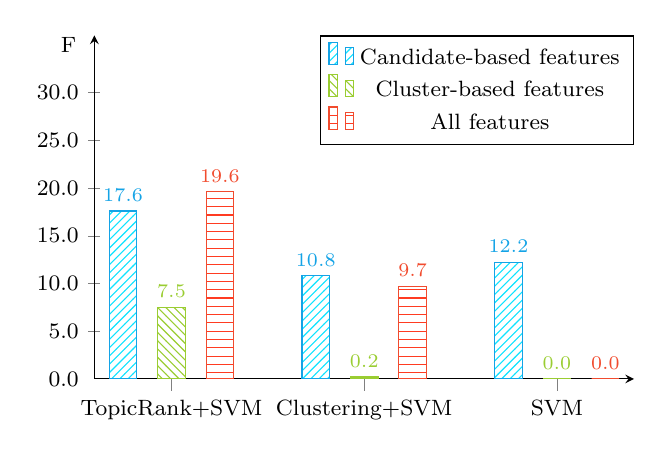
\begin{tikzpicture}
      \pgfkeys{/pgf/number format/.cd, fixed, fixed zerofill, precision=1}
      \begin{axis}[axis lines=left,
                   symbolic x coords={TopicRank+SVM, Clustering+SVM, SVM},
                   xtick=data,
                   enlarge x limits=0.2,
                   xticklabel style={font=\footnotesize},
                   nodes near coords,
                   nodes near coords align={vertical},
                   every node near coord/.append style={font=\scriptsize},
                   ytick={0.0, 5.0, 10.0, 15.0, 20.0, 25.0, 30.0},
                   yticklabel style={font=\footnotesize},
                   y=0.01\linewidth,
                   ymin=0.0,
                   ymax=36.0,
                   ybar=7.5pt,
                   ylabel=F,
                   ylabel style={at={(ticklabel* cs:1)},
                                 anchor=north east,
                                 yshift=.3em,
                                 xshift=.3em,
                                 rotate=270,
                                 font=\footnotesize},
                   legend style={at={(1.0, 1.0)},
                                 anchor=north east,
                                 font=\footnotesize}]
        \addplot[Cerulean,
                 pattern=north east lines,
                 pattern color=Cerulean] coordinates{
          (SVM, 12.2)
          (Clustering+SVM, 10.8)
          (TopicRank+SVM, 17.6)
        };
        \addplot[YellowGreen,
                 pattern=north west lines,
                 pattern color=YellowGreen] coordinates{
          (SVM, 0.0)
          (Clustering+SVM, 0.2)
          (TopicRank+SVM, 7.5)
        };
        \addplot[RedOrange,
                 pattern=horizontal lines,
                 pattern color=RedOrange] coordinates{
          (SVM, 0.0)
          (Clustering+SVM, 9.7)
          (TopicRank+SVM, 19.6)
        };
        \legend{Candidate-based features, Cluster-based features, All features}
      \end{axis}
    \end{tikzpicture}
    \caption{Performance of TopicRank+SVM$_{\text{all}}$ compared to derived
             baselines
             \label{fig:baseline_comparison}}
  \end{figure}

  Figure~\ref{fig:baseline_comparison} presents the performance of our method,
  compared to six baselines derived from it. On the first hand, we observe that
  using clusters and their importance score benefits to the keyphrase
  extraction. Most importantly, adding cluster-based features to the common
  features (candidate-based features) improves the performance. However, the
  performance achieved with the Clustering+SVM method shows that cluster-based
  features performs poorly when Topic\-Rank's importance score is not used.
  Additionally, the SVM performance tends to show that using clusters without
  taking their importance into account is not relevant. Results support our
  assumption that keyphrases should be extracted from important topics.

  \begin{table}
    \centering
    \begin{tabular}{|r|rrr|}
      \hline
      Method & \multicolumn{1}{c}{P} & \multicolumn{1}{c}{R} & \multicolumn{1}{c|}{F}\\
      \hline
      KEA                           & 18.8\textcolor{white}{$^\dagger$} & 13.3\textcolor{white}{$^\dagger$} & 15.4\textcolor{white}{$^\dagger$}\\
      TF-IDF                        & 13.2\textcolor{white}{$^\dagger$} & 8.9\textcolor{white}{$^\dagger$} & 10.5\textcolor{white}{$^\dagger$}\\
      TopicRank                     & 14.9\textcolor{white}{$^\dagger$} & 10.3\textcolor{white}{$^\dagger$} & 12.1\textcolor{white}{$^\dagger$}\\
      TopicRank+SVM$_{\text{all}}$  & 24.2$^\dagger$ & 16.7$^\dagger$ & 19.6$^\dagger$\\
      \hline
      TopicRank$_{\text{max}}$      & 37.6\textcolor{white}{$^\dagger$} & 25.8\textcolor{white}{$^\dagger$} & 30.3\textcolor{white}{$^\dagger$}\\
      \hline
    \end{tabular}
    \caption{Performance of TopicRank+SVM$_{\text{all}}$ compared to previous
             work. $\dagger$ indicates improvement over KEA, TF-IDF and
             TopicRank at 0.001 level using Student's t-test.
             \label{tab:state_of_the_art_comparison}}
  \end{table}

  Also, Table~\ref{tab:state_of_the_art_comparison} presents a comparison of
  TopicRank+SVM$_{\text{all}}$ with TopicRank, TopicRank's best possible
  performance (TopicRank$_{\text{max}}$) and common baselines of previous work.
  Results show that our method significantly improves TopicRank and
  significantly outperforms TF-IDF and KEA, a robust supervised methods.
  However, the performance of TopicRank+SVM$_{\text{all}}$ is still very low
  compared to TopicRank$_{\text{max}}$. The naivety of the clustering method
  TopicRank applies may introduce noise that dampens the performance. Future
  improvement should focus on a more efficient clustering of the candidates
  belonging to the same topic.

%\section{Example}
%\label{sec:example}


\section{Conclusion et perspectives}
\label{sec:conclusion_et_perspectives}
  Dans ce travail, nous proposons une méthode à base de graphe pour l'extraction
  non supervisée de termes-clés. Cette méthode groupe les termes-clés candidats
  en sujets, détermine quels sont ceux les plus importants, puis extrait le
  terme-clé candidat qui représente le mieux chacun des sujets les plus
  importants. Cette nouvelle méthode offre plusieurs avantages vis-à-vis des
  précédentes à base de graphe. Le groupement des termes-clés potentiels en
  sujets distincts permet de rassembler des indices utiles auparavant éparpillés
  et le choix d'un seul terme-clé pour représenter un sujet important permet
  d'extraire un ensemble de termes-clés non redondants ( pour $k$ termes-clés
  extraits, exactement $k$ sujets sont couverts). Enfin, le graphe est complet
  et ne requiert plus le paramétrage d'une fenêtre de cooccurrences,
  contrairement aux autres méthodes à base de graphe.

  Les bons résultats de notre méthode montrent la pertinence d'un groupement en
  sujets des candidats pour ensuite les ordonner. Les expériences
  supplémentaires montrent aussi qu'il est encore possible d'améliorer notre
  méthode en proposant une nouvelle stratégie de sélection du terme-clé candidat
  le plus représentatif d'un sujet (pour un gain maximum allant de 4,2 à 15
  points de f-score).

  Nous avons aussi effectué une analyse d'erreurs à partir de laquelle trois
  perspectives de travaux futurs émergent~:

  Nous avons pour objectif d'améliorer la sélection des termes-clés candidats.
  Aussi, des méthodes empruntées à d'autres domaines du TAL peuvent être
  appliquées. Il semble, par exemple, pertinent d'évaluer l'apport des méthodes
  d'extraction terminologiques~\cite{castellvi2001automatictermdetection} pour
  la sélection des termes-clés candidats.
  
  Nous envisageons également d'améliorer le groupement en sujets,
  car celui-ci est très naïf et ne tient compte ni de la synonymie, ni de
  l'ambiguïté des mots. De plus, l'usage du
  radical~\cite{porter1980suffixstripping} des mots n'est pas sans introduire du
  bruit lié à certains faux positifs (p.~ex. \og{}\underline{empir}e\fg{} et
  \og{}\underline{empir}ique\fg{}). L'ajout de connaissances concernant les
  synonymes permettrait de créer des sujets plus complets et une étape de
  désambiguïsation éviterait un groupement systématique des termes-clés
  candidats ayant un ou plusieurs mots en commun. Nous envisageons aussi de
  remplacer la racinisation de \newcite{porter1980suffixstripping} par une
  méthode de lemmatisation. D'un point de vue plus technique, il faudrait
  explorer différentes méthodes de groupement, dont le groupement spectral
  (\textit{spectral clustering}) qui, dans d'autres travaux portant sur
  l'extraction automatique de termes-clés~\cite{liu2009keycluster}, montre de
  meilleures performances que le groupement hiérarchique agglomératif.

  Enfin, une étude détaillée des caractéristiques des termes-clés pourrait
  orienter notre travail vers des critères plus efficaces pour la définition
  d'une stratégie \og{}optimale\fg{} de sélection du terme-clé le plus
  représentatif d'un sujet. Un apprentissage supervisé à partir de certains
  critères est aussi envisagé, au même titre que l'usage de méthodes
  d'optimisation, telles que celle utilisée par
  \newcite{ding2011binaryintegerprogramming} dans leur méthode d'extraction
  automatique de termes-clés.



\acknowledgements{
  Ce travail a bénéficié d'une aide de l'Agence Nationale de la Recherche
  portant la référence (ANR-12-CORD-0029).
}

\bibliography{../biblio}

\end{document}

